% English option set
\documentclass{VRARWorkshop}
\usepackage[utf8]{inputenc}
\usepackage[T1]{fontenc}
\usepackage{ngerman}
\usepackage[hidelinks]{hyperref}
% Define your paper's title. This has to be done BEFORE \begin{document}!
\title{Visual Raytrace: An Immersive Learning Application}

\authors{Manfred Brill, Benedict S"arota}


%\affiliations{~} %<---- anonymous submission
\affiliations{
    University of Applied Sciences Kaiserslautern \\
    Amerikastr. 1 \\
    66482 Zweibrücken \\
    Tel.: +49 (0)631 / 37 24 - [5382, 5321] \\
%    Fax: +49 (0)815 / 40 90 - 115 \\
    E-Mail: [manfred.brill, benedict.saerota]@hs-kl.de
}

\abstract{%
Visual Raytrace is an immersive learning application supporting students in a computer graphics class to create
their own version of a working raytracing software.
Users interact with the ingredients of a raytracer like coordinate systems, cameras, framebuffer, scene description,
sampling, reflection models or texture mapping.
}

% Give some keywords
\keywords{Virtual Reality, Immersive Learning, Computer Graphics,  Raytracing}

\graphicspath{{../figures/}} %Verzeichnis der Bitmaps

% Wir könnten ngerman weglassen weiter oben, aber dann bekommen wir Probleme
% mit dem Authorennamen Särota :-)
\usepackage[figurename=Figure]{caption}
\renewcommand{\refname}{References}
% Finally you get to work ;-) Start your document and...
\begin{document}
% ...begin with the introduction section right away. The title format
% will be generated automatically at the top of the page.

\section{Introduction}
Raytracing, introduced by Turner Whitted \cite{whitted_80}, is one of the major topics in
computer graphics classes.
In figure \ref{intro:whitted} we find one of the famous pictures rendered by Whitted.

\begin{figure}[h!]
    \begin{center}
        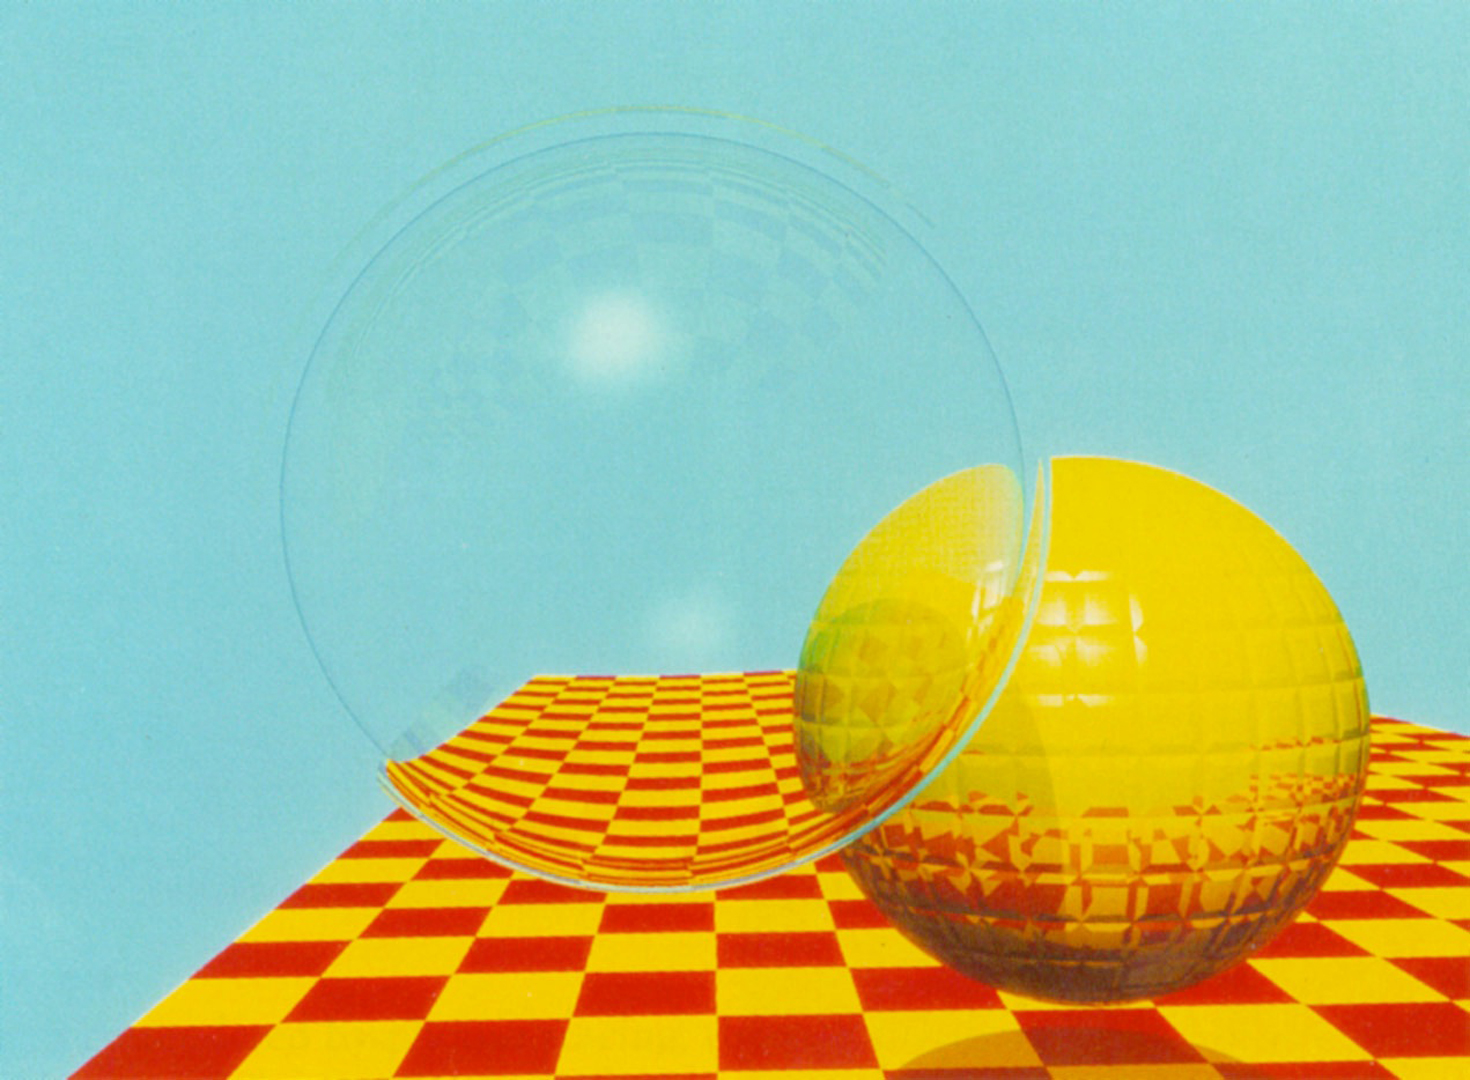
\includegraphics[width=0.35\textwidth]{whitted02.jpg}
        \caption{\label{intro:whitted} Image rendered by Turner Whitted \cite{checkerSpheres}}
    \end{center}
\end{figure}
Students in a computer graphics class usually implement their version of such a renderer
after being taught the theory in the class.
To achieve this they need to understand the basic concepts of computer graphics like coordinate systems,
cameras, reflection models or texture mapping. To implement a raytracer or another 3D application the students have to
develop strong visual thinking. Virtual reality applications provide joy of use and support the transfer
from 3D space to a programming language and deepen the understanding of the basic concepts of a raytracer.
%
\section{Visual Raytrace}
We implemented the immersive learning application \textbf{Visual Raytrace} \cite{saerota_21, visualraytrace} using the Unity Game Engine
and HTC Vive Input Utility \cite{viveInput}.
The application runs on HTC Vive Pro and Vive Focus Plus.
Figure \ref{vray:scene} shows the main features of the application.
The scene to be rendered is placed in the virtual environment as a world in a miniature \cite{pausch_95}.

\begin{figure}[h!]
    \begin{center}
        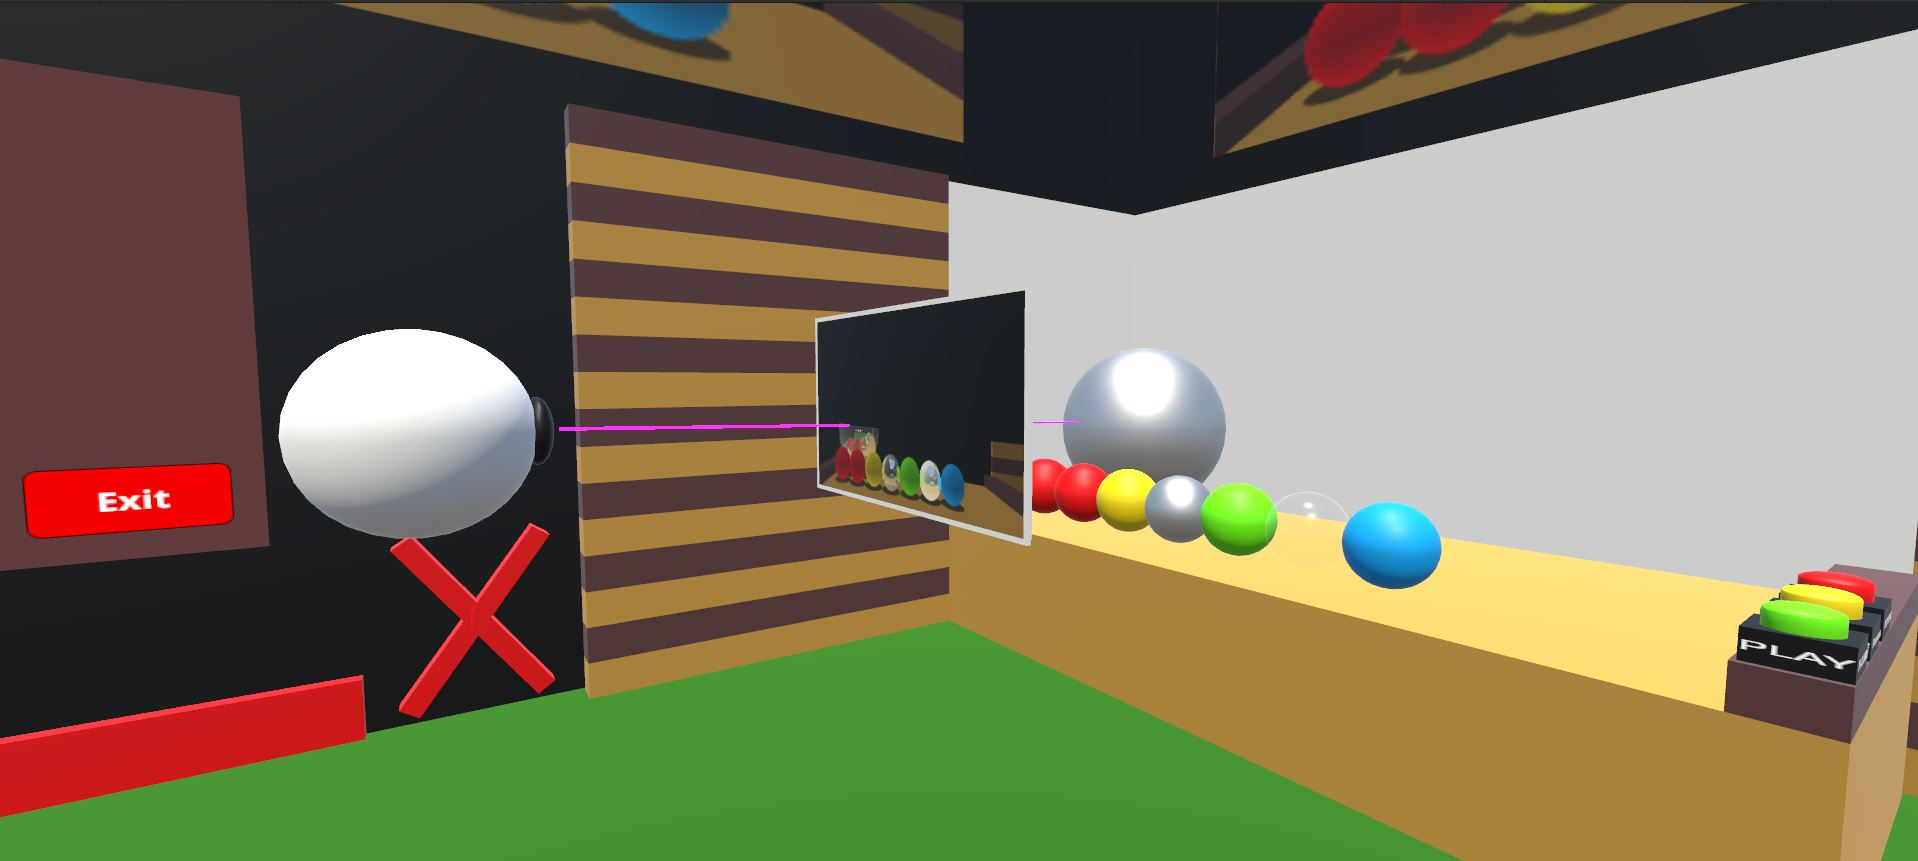
\includegraphics[width=0.55\textwidth]{duringProcess}
        \caption{\label{vray:scene} The elements of a raytracer in an immersive environment}
    \end{center}
\end{figure}
The raytracer is implemented in C\# and can be slowed down to make sure the users can follow the path
of the ray and the reflections in the scene until the color of the fragment is finally computed.
The raytracing process can be paused or stopped to get an understanding of the rendering algorithm.
At the end the computed image can be saved for further investigation.

\begin{figure}[h!]
    \begin{center}
        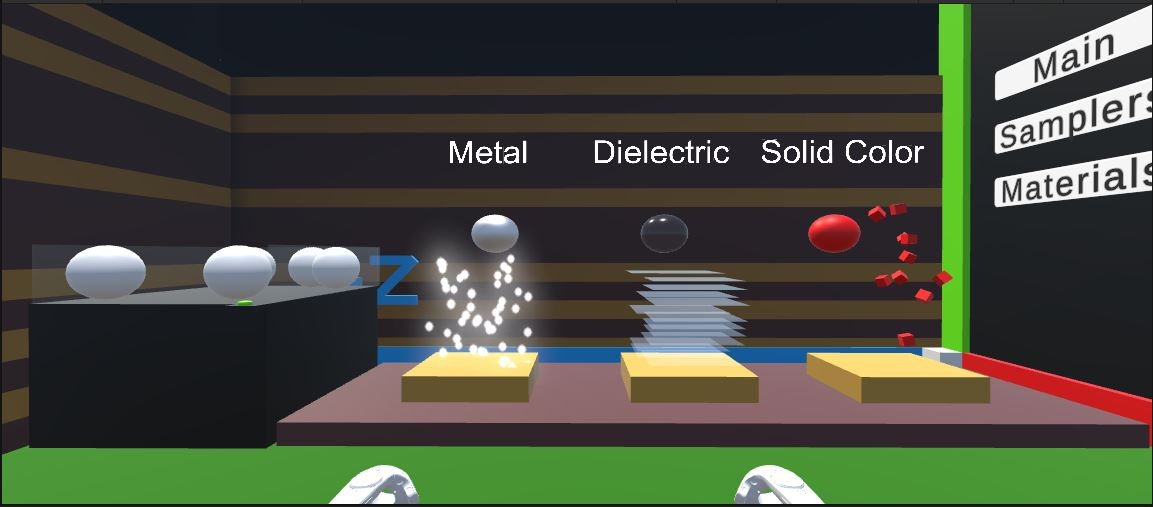
\includegraphics[width=0.55\textwidth]{sphereCreating}
        \caption{\label{vray:materials} Geometric objects and reflection functions for scene definition}
    \end{center}
\end{figure}
The raytracing scene can either be defined in VR or can be read from a scene description file.
Figure \ref{vray:materials} shows the interface for the interactive scene definition.
New objects can be picked, one of the reflection models can be assigned and the object
is then positioned in the raytracing scene.
The options for the raytracer can also be changed in the immersive environment.
%
\section{Future Work}
We plan to implement a change of scenes so the users can dive into the raytracing scene
and inspect the rendered scene or details of the rendering process.
We are working on builds for Google Cardboard, Oculus Android,
OpenXR and WebXR to support as many platforms as possible.

Due to the pandemic situation on our campus we could not evaluate the application with students.
Hopefully we will be able to do this in the winter term 2021/22 at our campus.
The results of this evaluation will help us to improve the usability and joy of use of the application.

We plan to use the immersive learning application in the next computer graphics class in our department
in summer 2022. The VR application will open up new ways of teaching \cite{ganovelli_08, vitsas_20}.
To support this we will transfer the C\# code for the raytracer to its own repository, so the raytracing code
can also be used stand-alone in the class.

%set appropriate bib style
\VRARsetbibstyle
\bibliography{paper}
\end{document}
